\newpage
\subsubsection*{Component-and-Connector View}

The view displays high-level communication between the subsystems and how they should work as a whole. Connections are defined by various communication channels and their protocols.
\vspace{3mm}

Apart from the usual interaction of the browser, web and back-end application trio, the Docker Swarm component introduces a few key interactions. The back-end application plays a key role as it queries resources from the database, while providing metrics via Serilog and DataDog Agent to the DataDog Logging Service. System telemetries are gathered and visualized with the interaction of Prometheus and Grafana. The metrics pulled from the back-end application by Prometheus are gathered by Grafana using PromQL. It is then displayed on dashboards for analysis.
\vspace{3mm}

\begin{figure}[h!]
    \centering
    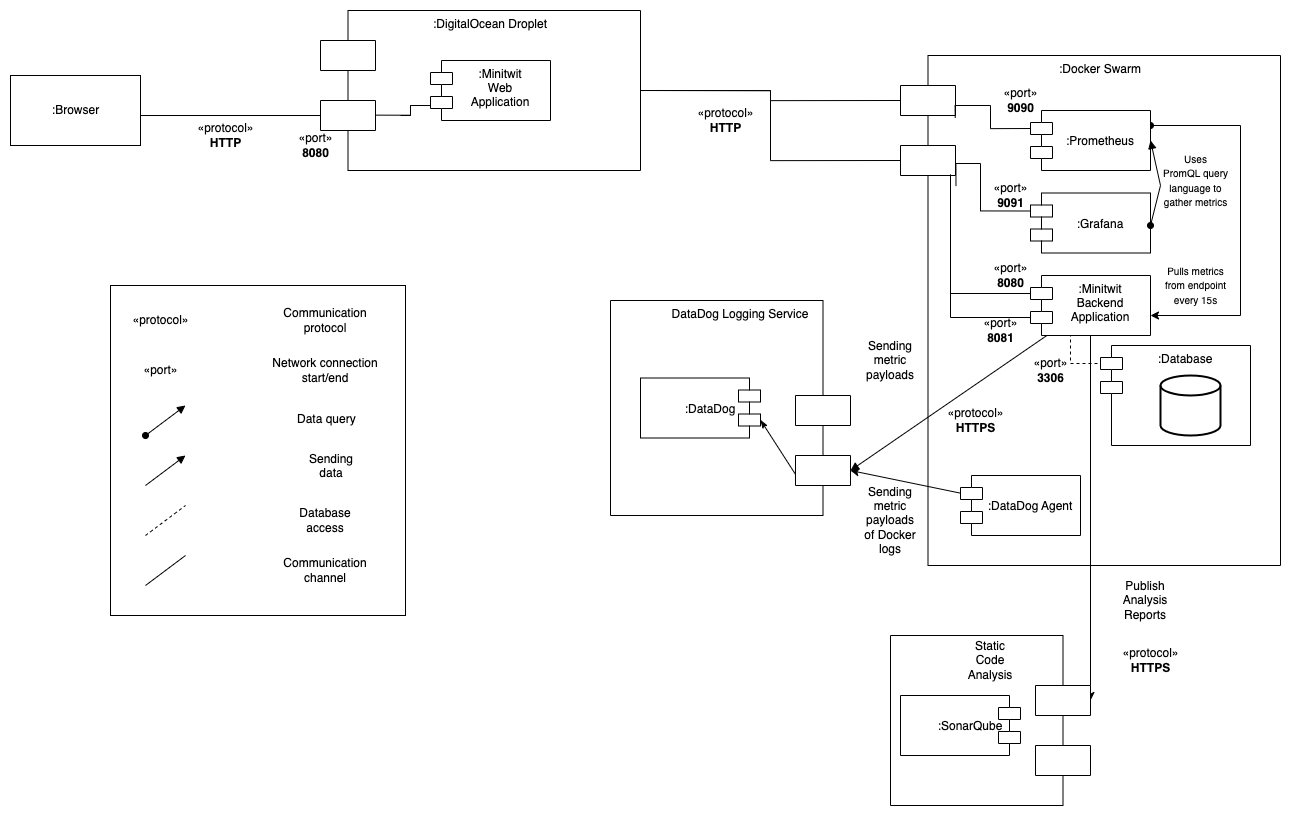
\includegraphics[width=\linewidth,height=\textheight,keepaspectratio]{images/architectural_views/minitwit_cc_view.png}
    \caption{Component-and-Connector View~\cite{componentAndConnectorView}.}
    \label{fig:ccview}
\end{figure}